%------------------------------------
% Dario Taraborelli
% Typesetting your academic CV in LaTeX
%
% URL: http://nitens.org/taraborelli/cvtex
% DISCLAIMER: This template is provided for free and without any guarantee 
% that it will correctly compile on your system if you have a non-standard  
% configuration.
% Some rights reserved: http://creativecommons.org/licenses/by-sa/3.0/
%------------------------------------

%!TEX TS-program = xelatex
%!TEX encoding = UTF-8 Unicode

\documentclass[11pt, letter]{article}
\usepackage{fontspec} 

% DOCUMENT LAYOUT
\usepackage{geometry} 
\geometry{a4paper, textwidth=5.5in, textheight=8.5in, marginparsep=7pt, marginparwidth=.6in}
\setlength\parindent{0in}
\usepackage[spanish]{babel}
\usepackage{graphicx}
% FONTS
\usepackage[usenames,dvipsnames]{xcolor}
\usepackage{xunicode}
\usepackage{xltxtra}
\defaultfontfeatures{Mapping=tex-text}
%\setromanfont [Ligatures={Common}, Numbers={OldStyle}, Variant=01]{Linux Libertine O}
%\setmonofont[Scale=0.8]{Monaco}
%%% modified by Karol Kozioł for ShareLaTeX use
\setmainfont[
  Ligatures={Common}, Numbers={OldStyle}, Variant=01,
  BoldFont=LinLibertine_RB.otf,
  ItalicFont=LinLibertine_RI.otf,
  BoldItalicFont=LinLibertine_RBI.otf
]{LinLibertine_R.otf}
\setmonofont[Scale=0.8]{DejaVuSansMono.ttf}
\setsansfont{Latin Modern Sans}

% ---- CUSTOM COMMANDS
\chardef\&="E050
\newcommand{\html}[1]{\href{#1}{\scriptsize\textsc{[html]}}}
\newcommand{\pdf}[1]{\href{#1}{\scriptsize\textsc{[pdf]}}}
\newcommand{\doi}[1]{\href{#1}{\scriptsize\textsc{[doi]}}}
% ---- MARGIN YEARS
\usepackage{marginnote}
\newcommand{\amper{}}{\chardef\amper="E0BD }
\newcommand{\years}[1]{\marginnote{\scriptsize #1}}
\renewcommand*{\raggedleftmarginnote}{}
\setlength{\marginparsep}{7pt}
\reversemarginpar

% HEADINGS
\usepackage{sectsty} 
\usepackage[normalem]{ulem}
\sectionfont{\mdseries\upshape\Large}
\subsectionfont{\mdseries\scshape\normalsize} 
\subsubsectionfont{\mdseries\upshape\large} 

% PDF SETUP
% ---- FILL IN HERE THE DOC TITLE AND AUTHOR
\usepackage[%dvipdfm, 
bookmarks, colorlinks, breaklinks, 
% ---- FILL IN HERE THE TITLE AND AUTHOR
	pdftitle={Gerardo Mart\'in - vita},
	pdfauthor={Gerardo},
	%pdfproducer={http://nitens.org/taraborelli/cvtex}
]{hyperref}  
\hypersetup{linkcolor=blue,citecolor=blue,filecolor=black,urlcolor=MidnightBlue} 

\usepackage{multicol}

%ORCID
\usepackage{tikz,xcolor,hyperref}

% Make Orcid icon
\definecolor{lime}{HTML}{A6CE39}
\DeclareRobustCommand{\orcidicon}{%
	\begin{tikzpicture}
	\draw[lime, fill=lime] (0,0) 
	circle [radius=0.18] 
	node[white] {{\fontfamily{lmss}\selectfont \tiny ID}};
	\draw[white, fill=white] (-0.0825,0.099) 
	circle [radius=0.007];
	\end{tikzpicture}
	\hspace{-2mm}
}

\foreach \x in {A, ..., Z}{%
	\expandafter\xdef\csname orcid\x\endcsname{\noexpand\href{https://orcid.org/\csname orcidauthor\x\endcsname}{\noexpand\orcidicon}}
}

\newcommand{\orcidauthorA}{0000-0003-3608-5328}

% DOCUMENT
\begin{document}

{\LARGE Gerardo Antonio Mart\'in Mu\~noz de Cote \orcidA{}}\\ [0.5cm]
{\small PhD., MSc. Biol. Cons., MVZ. --- SNI I}\\[0.5cm]
{\large Curriculumvit\ae}\\
{\small \today}\\[0.5cm]

\begin{multicols}{2}
\begin{center}
	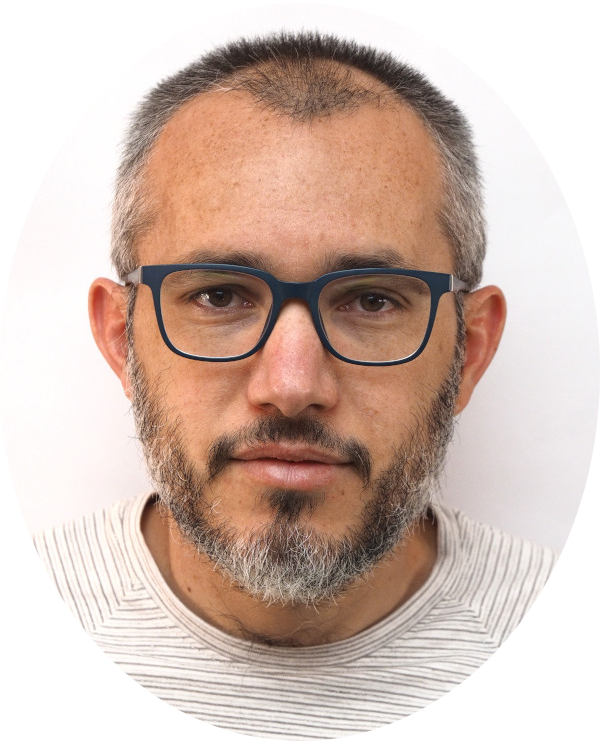
\includegraphics[width=.7\linewidth]{yo}
\end{center}

2$^a$ Privada Mapim\'i 610, Colonia Hip\'odromo\\
Durango, DGO\\
M\'exico\\[.2cm]
M\'ovil: \texttt{(+52) 618 116 82-37}\\
Whatsapp: \texttt{(+52) 618 116 82-37}\\
E-mail:
\begin{description}
	\item[Personal:] \href{mailto:gerardommc@gmail.com}{gerardommc@gmail.com}
	\item[Institucional:] \href{mailto:gerardo.mmc@enesmerida.unam.mx}{gerardo.mmc@enesmerida.unam.mx}
\end{description}
Fecha de nacimiento:  2 de marzo de 1981---Oxford, Inglaterra\\
Nacionalidad:  Mexicano

\end{multicols}

\vspace{1.5cm}

%%\hrule
\section*{\'Areas de especializaci\'on}
Modelado espacial de procesos ecol\'ogicos y transmisi\'on de enfermedades $ \bullet $ Estad\'istica espacial $ \bullet $ Problemas inversos aplicados en ecolog\'ia $ \bullet $ Biolog\'ia de Conservaci\'on $ \bullet $ Ecolog\'ia de enfermedades infecciosas $ \bullet $ Aplicaciones ecol\'ogicas en salud p\'ublica $ \bullet $ Eco-epidemiolog\'ia

\section*{Educaci\'on}

\years{2012-2016} Doctorado en Filosof\'ia. College of public health, medical and veterinary sciences, James Cook University. Fecha de obtenci\'on del grado: 22 de mayo de 2017. Con la tesis:
\textbf{Modelling Hendra virus transmission from flying foxes to horses}.\\

\years{2007-2010} Maestr\'ia en Ciencias, Biolog\'ia de la Conservaci\'on, Instituto de Ecolog\'ia A.C. Con la tesis:
\textbf{Modelo de leptospirosis y comparaci\'on de su frecuencia entre la ardilla de Perote (\emph{Spermophilus perotensis}), y dos especies dom\'esticas}.\\

\years{2001-2006} Licenciatura en Medicina Veterinaria y Zootecnia, Universidad de LaSalle Baj\'io. Promedio final de 9.5\\

\years{2000-2001} 1er a\~no de Ciencias de Computaci\'on, Facultad de Matem\'aticas, Universidad de Guanajuato.\\

\section*{Experiencia profesional}

\years{2021-} Profesor asociado C de tiempo completo. Escuela Nacional de Estudios Superiores unidad Mérida.

\years{2020-2021} Investigador posdoctoral DGAPA\footnote{\url{https://dgapa.unam.mx/}}, Escuela Nacional de Estudios Superiores unidad M\'erida, Universidad Nacional Aut\'onoma de M\'exico. Proyecto: 

\begin{itemize}
\item Nichos ecol\'ogicos fundamentales: supuestos estad\'isticos y alternativas geo-estad\'isticas para estimarlos
\end{itemize}

\years{2020} Profesor de asignaturas en la Facultad de Medicina Veterinaria y Zootecnia, Universidad Juárea del Estado de Durango:
\begin{itemize}
 \item Estad\'istica 1
 \item Patolog\'ia general
\end{itemize}

\years{2018-2020} Investigador asociado (Post-doc). Ecological Health Research Group (\href{http://murraylab.weebly.com/}{Murray Lab}\footnote{\url{http://murraylab.weebly.com/}}),  Department of Infectious Disease Epidemiology, Faculty of Medicine, Imperial College London at St. Mary's.\\

\years{2017} Consultor analista para el proyecto \lq \lq Modeling Spillover\rq \rq. Bozeman Disease Ecology Lab, Montana State University. Responsable del proyecto: Raina K. Plowright.\\

\years{2012-2016} Investigaci\'on (Candidato a Doctor en Filosof\'ia), James Cook University, Townsville, QLD, AU.\\

\years{2007-2010} Investigaci\'on (Candidato a Maestro en Ciencias). Instituto de Ecolog\'ia, Xalapa, Ver, Mex.\\

\years{2007} Practicante de medicina de peque\~nas especies.\\

\years{2006}  Pr\'acticas profesionales. Durrell Wildlife Conservation Trust, Jersey Zoo, Jersey, Channel Islands. Responsable: M.Sc. Javier L\'opez, jefe del departamento de servicios veterinarios. Desarroll\'e el proyecto de investigaci\'on: \lq \lq A pilot study on the anaesthtic effects of the combination of Ketamine – medetomidine, and propofol in the anuran \emph{Polypedates leucomystax}\rq \rq.\\

\years{2006} 600 h de servicio social profesional. Laboratorio de patolog\'ia animal, Uni\'on Ganadera Regional, Le\'on, Guanajuato, Mex. Responsable: M.V.Z. Manuel Conrado Gonz\'alez, Jefe del Laboratorio de Patolog\'ia. \\

\subsection*{Experiencia docente}

%\years{2022} Estancia de Investigación. Licenciatura en Manejo Sustentable de la Zona Costera. ENES M\'erida, UNAM.\\

\years{2022} Estad\'istica Multivariada. Licenciatura en Manejo Sustentable de Zonas Costeras. ENES M\'erida, UNAM.\\

\years{2022} M\'etodos de Campo y Laboratorio. Licenciatura en Manejo Sustentable de Zonas Costeras. ENES M\'erida, UNAM.\\

\years{2022} Introducci\'on a la Estad\'istica. Licenciatura en Ciencias Ambientales. ENES M\'erida, UNAM.\\

\years{2022} Modelaci\'on Matem\'atica. Licenciatura en Ciencias Ambientales. ENES M\'erida, UNAM.\\

\years{2022} Modelos Matem\'aticos en Ecolog\'ia I. Licenciatura en Ecolog\'a. ENES M\'erida, UNAM.\\

\years{2022} Modelado y Análisis Espacial. Licenciatura en Ciencias Ambientales. ENES M\'erida, UNAM.\\

\years{2021} Modelos Matem\'aticos en Ecolog\'ia. Licenciatura en Ecolog\'a. ENES M\'erida, UNAM.\\

\years{2021} Modelaci\'on Matem\'atica. Licenciatura en Ciencias Ambientales. ENES M\'erida, UNAM.\\

\years{2021} Planeación y análisis de experimentos. Licenciatura en Manejo sustentable de la zona costera. ENES Mérida, UNAM.\\

\years{2020} Estad\'istica I y Patolog\'ia general - Facultad de Medicina Veterinaria y Zootecnia, Universidad Ju\'arez del Estado de Durango.\\

\years{2018-} Supervisor de proyecto de investigaci\'on en el programa \lq\lq Masters of Environmental Technology\rq\rq\, Imperial College London de Tenghua Huang.\\

\years{2018-2019} Ayudant\'ia de estudiantes de doctorado en Imperial College London\footnote{\href{mailto:p.huxley@imperial.ac.uk}{Paul J. Huxley} y \href{mailto:h.shah16@imperial.ac.uk}{Hiral Shah}}.\\

\years{2018-} Impartici\'on del curso: \lq\lq Modelando el espacio para modelar los nichos ecol\'ogicos con herramientas frecuentistas y bayesianas\rq\rq. Escuela Nacional de Estudios Superiores unidad M\'erida, Parque Cient\'ifico y Tecnol\'ogico de Yucat\'an. 5 de noviembre de 2018.

%\hrule
\section*{Proyectos, becas y reconocimientos}
\noindent

\years{2022-2023} Responsable de proyecto PAPIIT IA200822 \lq\lq Estimaci\'on estad\'istica de nichos ecol\'ogicos y aplicaciones ecol\'ogicas, salud p\'ublica y conservaci\'on\rq\rq. \\

\years{2020-2021} Beca DGAPA para investigación posdoctoral en la Escuela Nacional de Estudios Superiores unidad Mérida, UNAM.\\

\years{2012-2016} Beca para investigaci\'on del National Hendra Virus Research Program, Australia. RIRDC PRJ-008213 (Models that predict Hendra virus transmission from flying foxes to horses).\\

\years{2010} Premio \emph{Bernardo Villa} en el primer congreso Latinoamericano de Mastozoolog\'ia. Primer lugar en la categor\'ia de excelencia a la mejor tesis de Maestr\'ia.\\

\section*{Publicaciones y pl\'aticas}

\subsection*{Art\'iculos en revistas arbitradas}

\years{2022} Jos\'e Mar\'ia Guti\'errez, Juliette Borri, Tamara Giles-Vernick, Romain Duda, Abdurazaq Habib, Anita Malhotra, \textbf{Gerardo Mart\'in}, Anna F. V. Pintor, Julien Potet, Terrence Scott, Isabelle Bolon, \& Rafael Ruiz Cata\~neda. Understanding and tackling snakebite envenoming with transdisciplinary research. \emph{PLoS Neglected Tropical Diseases}. ISSN: 1935-2735. \emph{En prensa}. \\

\years{2022} \textbf{Gerardo Mart\'in}, Joseph J. Erinjery, Dileepa Ediriweera, David G. Lalloo, H. Janaka de Silva, Takuya Iwamura \& Kris A. Murray. A mechanistic model of snakebite as a zoonosis: envenoming incidence is driven by snake ecology, socioeconomics and its impacts on snakes. \emph{PLoS Neglected Tropical Diseases}. ISSN: 1935-2735. \url{http://dx.doi.org/10.1371/journal.pntd.0009867}.\\

\years{2022} \textbf{Gerardo Mart\'in}, Carlos Y\'a\~nez Arenas \& Xavier Chiappa Carrara. Discrepancies between point process models and environmental envelopes identify the niche centroid-geography configuration. \emph{Ecological Modelling}. ISSN: 0304-3800. \url{https://doi.org/10.1016/j.ecolmodel.2022.109974}.\\

\years{2021} \textbf{Gerardo Mart\'in}, Joseph Erinjery, Rikki Gumbs, Ruchira Somaweera, Dileepa Ediriweera, Peter J. Diggle, Anuradhani Kasturiratne, Janaka de Silva, David G. Lalloo, Takuya Iwamura \& Kris A. Murray. Integrating snake distribution, abundance and expert-derived behavioural traits predicts snakebite risk. \emph{Journal of Applied Ecology}. ISSN: 1365-2664. \url{https://doi.org/10.1111/1365-2664.14081}.\\

\years{2021} \textbf{Gerardo Mart\'in}, Joseph Erinjery, Dileepa Ediriweera, David G. Lalloo, Takuya Iwamura \& Kris A. Murray. Redefining snakebite as a zoonosis: disease incidence is driven by snake ecology, socioeconomics and anthropogenic impacts. \emph{MedRXiv}. \url{https://doi.org/10.1101/2021.10.01.21264438}.\\

\years{2021} \textbf{Gerardo Martín}, Carlos Y\'a\~nez-Arenas, Rodrigo S. Camacho, Eyal Goldstein, Takuya Iwamura, Kris A. Murray \& Xavier Chiappa-Carrara. Implications of global environmental change for the burden of snakebite. \emph{ToxiconX}. ISSN: 2590-1710. \url{https://doi.org/10.1016/j.toxcx.2021.100069}.\\

\years{2021} Eyal Goldstein,Joseph Erinjery, \textbf{Gerardo, Mart\'in}; Anuradhani Kasturiratne, Dileepa Ediriweera, Janaka de Silva, Peter J. Diggle, Peter, David G. Lalloo, Kris A. Murray, \& Takyua Iwamura. \textbf{Integrating human behavior and snake ecology with agent-based models to predict snakebite in high risk landscapes}. \emph{PLoS Neglected Tropical Diseases}. ISSN: 1935-2735. \url{https://doi.org/10.1371/journal.pntd.0009047}.\\

\years{2020} Carlos Y\'a\~nez-Arenas, \textbf{Gerardo Mart\'in}, Luis Osorio-Olvera, Jazm\'in Escobar-Luj\'an, Sandra Casta\~no-Quintero \& Enrique Mart\'inez-Meyer. \textbf{The niche centrality hypothesis: key points about unfilled niches and the potential use of supraspecific modeling units}. \emph{Biodiversity Informatics}.\\

\years{2020} \textbf{Gerardo Mart\'in}, Mario Espinoza, Michelle Heupel, \& Colin Simpfendorfer. \textbf{Estimating marine protected area network benefits for reef sharks}. \emph{Journal of Applied Ecology}. eISSN: 1365-2664. \url{https://doi.org/10.1111/1365-2664.13706}. \href{https://besjournals.onlinelibrary.wiley.com/doi/toc/10.1111/(ISSN)1365-2664.Southwood_Prize_2020}{Nominado al premio Southwood 2020 a mejor artículo de la revista}.\\

\years{2019} Kris Murray, \textbf{Gerardo Mart\'in} \& Takuya Iwamura. \textbf{Focus on snake ecology to fight snakebite}. \emph{The Lancet}. (19) 325. ISSN: 01406736. \url{https://doi.org/10.1016/S0140-6736(19)32510-3}\\

\years{2018} \textbf{Gerardo Mart\'in}; Becker, Daniel; Washburn, Alex \& Raina K. Plowright. \textbf{Environmental persistence of influenza H5N1 is driven by temperature and salinity: insights from a Bayesian meta-analysis}. \emph{Frontiers in Ecology and Evolution}. eISSN: 2296701X. \url{https://doi.org/10.3389/fevo.2018.00131}\\

\years{2018} Brannelly, Laura A.; \textbf{Gerardo Mart\'in}; Lewellyn, John; Skerratt, Lee \& Lee Berger. \textbf{Size dependant susceptibility to chytridiomycosis in the invasive \emph{Rhinella marina}}. \emph{Diseases of Aquatic Organisms}. 131:107-120. ISSN: 01775103. eISSN: 16161580. \url{ https://doi.org/10.3354/dao03278}.\\

\years{2018} \textbf{Gerardo Mart\'in}; Y\'a\~nez-Arenas, Carlos; Plowright, Raina K.; Carla Chen \& Skerratt, Lee. \textbf{Hendra virus spillover is a bimodal system driven by climatic factors}. \emph{EcoHealth}. 15: 526–542. ISSN: 16129202. eISSN: 16129210. \url{https://doi.org/10.1007/s10393-017-1309-y}.\\

\years{2018} \textbf{Gerardo Mart\'in}; Y\'a\~nez-Arenas, Carlos; Plowright, Raina K.; Carla Chen \& Skerratt, Lee. \textbf{Climate change could increase the extent of areas at risk of Hendra virus spillover}. \emph{EcoHealth}. 15: 509–525. ISSN: 16129202. eISSN: 16129210. \url{https://doi.org/10.1007/s10393-018-1322-9}.\\

\years{2017} Carlos Alberto Y\'a\~nez-Arenas, Rodolfo Rioja-Nieto, Flipe Dzul-Manzanilla, \textbf{Gerardo Mart\'in}, Xavier Chiappa-Carrara, Aura Buenfil-\'Avila, Pablo Manrique-Saide, Fabi\'an Correa-Morales, Jos\'e Alberto D\'iaz-Qui\~n\'onez, Cresecencio P\'erez-Renter\'ia, Jos\'e Ordo\~nez-\'Alvarez \& Her\'on Huerta. \textbf{Characterization of environmental suitability for the Asian tiger mosquito (\emph{Aedes albopictus}) in M\'exico}. \emph{Journal of Medical Entomology}. ISSN: 19382928. eISSN: 00222585. 55(1):69–77. \url{https://doi.org/10.1093/jme/tjx185}\\

\years{2017} \textbf{Gerardo Mart\'in}, Rebecca J. Webb, Raina K. Plowright, Carla Chen, \& Lee F. Skerratt. \textbf{Microclimates might limit indirect spillover of the bat borne zoonotic Hendra virus}. \emph{Microbial ecology}. 74: 106–115. ISSN: 1432184X. \url{https://doi.org/10.1007/s00248-017-0934-x}.\\

\years{2016} \textbf{Gerardo Mart\'in}, Lee F. Skerratt, Carlos Y\'a\~nez-Arenas, Raina K. Plowright \& Carla Chen. \textbf{Climatic suitability influences species specific abundance patterns of Australian flying foxes and risk of Hendra virus spillover}. \emph{One Health Journal}. 2: 115-121. ISSN: 23527714. \url{https://doi.org/10.1016/j.onehlt.2016.07.004}.\\

\years{2016} Alison J. Peel, Hume E. Field, Peter A. Reid, Raina K. Plowright, Christopher C. Broder, Lee F. Skerratt, David T. S. Hayman, Olivier Restif, Melanie Taylor, \textbf{Gerardo Mart\'in}, Gary Crameri, Ina Smith, Michelle Baker, Glenn A. Marsh, Jennifer Barr, Andrew C. Breed, James L. N. Wood, Navneet Dhand, Jenny-Ann Toribio, Andrew A. Cunningham, Ian Fulton, Wayne L. Bryden, Cristy Secombe, Lin-Fa Wang. \textbf{The equine Hendra virus vaccine remains a highly effective preventative measure against infection in horses and humans: \lq The imperative to develop a human vaccine for the Hendra virus in Australia\rq\.} \emph{Infection Ecology and Epidemiology}. 6(1):31658. ISSN: 20008686. \url{https://doi.org/10.3402/iee.v6.31658}.\\

\years{2015} \textbf{Gerardo Mart\'in}, Raina K. Plowright, Carla Chen, Carla, David Kault, Paul Selleck \& Lee F. Skerratt. \textbf{Hendra virus survival does not explain the pattern of transmission and implicates relatively direct transmission routes}. \emph{Journal of General Virology}. 96(6). ISSN: 00221317. eISSN: 14652099. \url{https://doi.org/10.1099/vir.0.000073}.\\

\years{2015} Raina K. Plowright, Peggy Eby, Peter Hudson,Ina Smith, David Westcott, Wayne Bryden, Deborah Middleton, Peter Reid, Rosemary McFarlane, \textbf{Gerardo Mart\'in}, Gary Tabor, Lee Skerratt, Dale Anderson, Gary Crameri, David Quammen, David Jordan, Paul Freeman, Lin-Fa Wang, Jonathan Epstein, Glenn Marsh, Nina Kung \& Hamish McCallum. \textbf{Ecological Dynamics of Emerging Bat Virus Spillover}. \emph{Proceedings of the Royal Society B}.  282(1798). ISSN: 09628452. \url{https://doi.org/10.1098/rspb.2014.2124}.\\

\years{2013} Rosaura Valdez-Lares, \textbf{Gerardo A. Mart\'in-Mu\~noz de }, Ra\'ul Mu\~niz-Mart\'inez \& Georgina Santos-Barrera. \textbf{New distributional records for amphibians from Durango, M\'exico}. \emph{Herpetological Review}. 44 (4): 646-649. ISSN: 0018084X. \url{https://bit.ly/2zIsM3R}.\\

\subsubsection*{Art\'iculos en revisión}

\years{2022} Joseph J. Erinjery, Eyal Golstein, \textbf{Gerardo Mart\'in}, et al. \textbf{Land use change in Sri Lanka during the armed conflict}. \emph{Journal of Land Use Policy}. \\

\years{2022} Eyal Golstein, Joseph J. Erinjery, \textbf{Gerardo Mart\'in}, et al. \textbf{Farmers adaptation to climate uncertainty as drivers of snakebite risk}. \emph{Nature communications}.\\

\subsubsection*{Art\'iculos en preparaci\'on}

\years{2022}  \textbf{Gerardo Mart\'in}, Joseph Erinjery, Eyal Goldstein, Takuya Iwamura \& Kris Murray. \textbf{Global change projections for snakebite incidence in South Asia: Conflicts between public health and conservation objectives}.\\

\years{2022} 	Joseph J. Erinjery, \textbf{Gerardo Mart\'in}, Eyal Goldstein, Kris Murray \& Takuya Iwamura. \textbf{Global change predictions based on socioeconomic pathways for Sri Lanka}.\\

\subsubsection*{Investigaciones en curso}

\begin{itemize}
	
	\item Tiffany Kosch, \& \textbf{Gerardo Mart\'in}. \textbf{Modelling the prevalence of amphibian chytridiomycosis in Peru}.\\
	
	\item \textbf{Gerardo Mart\'in}, John R. Giles, David Westcott, Hazel Parry, Raina Plowright, Raina, Carla Chen \& Lee F. Skerratt. \textbf{Landscape level mechanisms driving risk of Hendra virus spillover}.\\
\end{itemize}


\subsection*{Art\'iculos de divulgaci\'on}

\years{2021} Gerardo Mart\'in. \textbf{Integrating snake distribution, abundance and expert-derived behavioural traits to predict snakebite risk}. \href{https://appliedecologistsblog.com/2021/12/27/integrating-snake-distribution-abundance-and-expert-derived-behavioural-traits-to-predict-snakebite-risk/}{\emph{The Applied Ecologist}}.\\

\years{2020} Colin Simpfendorfer \& Gerardo Mart\'in. \textbf{Protected high-value reefs and movement pathways improve conservation of reef sharks}. \href{https://appliedecologistsblog.com/2020/07/30/protected-high-value-reefs-and-movement-pathways-improve-conservation-of-reef-sharks/}{\emph{The Applied Ecologist}}.\\

\years{2013} Jon Luly, Gerardo Mart\'in Lee Skerratt. 30 April 2013. \textbf{Breaking up bat colonies doesn't eliminate health risks}. \href{http://theconversation.com/breaking-up-bat-colonies-doesnt-eliminate-health-risks-13580}{\emph{The Conversation}}


\subsection*{Pl\'aticas y p\'osters}

\years{2022} Congreso Científico Mexicano de Ecología, Oaxaca, Oax.

\begin{enumerate}
	\item Presentación oral: \textbf{Identificando la configuración geográfico-ambiental de los nichos ecológicos}
	\item Poster: \textbf{El ofidismo como un proceso dinámico ante el cambio global}
	\item Poster: \textbf{Modelos de agentes para optimizar la protección de tiburones de arrecife en redes de áreas naturales}
\end{enumerate}

\years{2020} Seminario Institucional, ENES Mérida. \textbf{Puentes cuantitativos entre medicina y ecología}. \\

\years{2019} Association for Tropical Biology and Conservation, Asia-Pacific Chapter, Thulhiriya, Sri Lanka. \textbf{Abundance of venomous snakes of Sri Lanka in relation to climate and land cover}.\\

\years{2019} MRC seminar, winter series, Imperial College London at St. Mary's. \textbf{Modelling the effects of global change on snakebite burden}.\\

\years{2017} Seminarios Institucionales, Departamento de Biolog\'ia, Universidad de Guanajuato. \textbf{Ecolog\'ia de enfermedades infecciosas: ¿una quimera de la biolog\'ia?}\\

\years{2017} WDA international conference, San Crist\'obal de las Casas, Chiapas. \textbf{Ecological niche modelling studies of Hendra virus spillover}. Pl\'atica.\\

\years{2017} Coloquio CIMAT. \textbf{Modelos para entender y predecir la diseminaci\'on de pat\'ogenos}. Seminario.\\

\years{2016} One Health Symposium. Division of Tropical Health and Medicine, College of Public Health, Medical and Veterinary Sciences, James Cook University. \textbf{Models that predict the risk of Hendra virus transmission from flying foxes to horses}. Pl\'atica.\\

\years{2016} CBMDT and CBTID, College of Public Health, Medical and Veterinary Sciences Fitzroy island retreat. \textbf{Models of Hendra virus survival to infer transmission pathways from bats to horses}. Pl\'atica.\\

\years{2016} CBMDT and CBTID, College of Public Health, Medical and Veterinary Sciences Fitzroy island retreat. \textbf{Models that predict risk of Hendra virus transmission from flying foxes to horses}. P\'oster.\\

\years{2015} Wildlife Disease Association 2015 International Conference, Maroochydore, QLD, Australia. \textbf{Understanding frequency of contact between horses and Hendra virus}. P\'oster.\\

\years{2014} Australasian Bat Society 2014 Conference. Townsville, QLD, Australia. \textbf{Hendra virus risk of spillover: The effect of weather and climate}. Pl\'atica.\\

\years{2013} Wildlife Diseases Association Australasian section 2013 Conference. Grampians, VIC, Australia. \textbf{Contribution of climate and weather to the distribution of Hendra virus spillover events}. Pl\'atica.\\

\years{2010} 10$^o$ Congreso Nacional y 1$^{er}$ Congreso Latinoamericano de Mastozoolog\'ia, Guanajuato, Gto., Mexico. \textbf{Modelo de leptospirosis y comparaci\'on de sufrecuencia entre dos sitios en la ardilla de Perote (\emph{Spermophilus 
		perotensis}) y dos especies dom\'esticas}. Pl\'atica.\\

\years{2009} 1$^{er}$ Congreso Nacional de Ecolog\'ia de Enfermedades Infecciosas y Medicina de la Conservaci\'on, Veracruz, Ver., Mexico. \textbf{Modelo de leptospirosis y comparaci\'on de sufrecuencia entre dos sitios en la ardilla de Perote (\emph{Spermophilus perotensis}) y dos especies dom\'esticas}. Pl\'atica.\\

\section*{Proyectos financiados}

\subsection*{Como responsable}

\years{2021} Estimación estadística de nichos ecológicos y aplicaciones ecológicas, salud pública y conservación, PAPIIT-UNAM, IA200822.

\subsection*{Como participante}

\years{2018} The dynamic challenge of snakebite in South Asia. Medical Research Council UK.\\

\years{2017} Predicting pathogen spillover. US Ministry of Defense.\\

\years{2012} Modelling Hendra virus transmission from flying foxes to horses. Rural Industries Research and Development Coporation, AU.

\section*{Educaci\'on cont\'inua}

\years{2018} Software carpentry workshop---git, linux shell). Imperial College London, South Kensington.\\

\years{2015} Workshop for advanced techniques in data analysis with R. James Cook University. Townsville, QLD, AU. Dr. Murray Logan.\\

\years{2014} 2$^{\mathrm{nd}}$ Thematic school \lq\lq Ecology, Evolution and Control of Infectious Diseases. Laboratory of Excellence CEBA. M\'erida, Yuc., MX. Dr. Jean Fran\c{c}ois Gu\'egan y ponentes varios. \\

\years{2013} Infectious disease modelling workshop. Ausralian Mathematical Sciences Institute. Newcastle, NSW, AU. Ponentes varios\\

\years{2011} Escuela de Modelaci\'on y M\'etodos Num\'ericos. CIMAT A.C. Guanajuato, Gto., MX. Profesores varios.\\

\years{2011} Taller de sistemas de informaci\'on geogr\'afica. CIIDIR-IPN. Durango, Dgo., MX. Dr. Armando Uribe-Contreras.\\

\years{2008} T\'ecnicas para el estudio de la fauna silvestre. INECOL A.C. Reserva de la bi\'osfera de Mapim\'i. Dra. Sonia Gallina Tessaro.\\

\years{2006} De Darwin a la gen\'etica evolutiva. Universidad de Guanajuato, Museo Alfredo Dug\'es. Guanajuato, Gto., MX.

\section*{Revisi\'on para revistas acad\'emicas}

\begin{itemize}
 \item Scientific Data
 \item PLoS Neglected Tropical Diseases
 \item Acta Zool\'ogica Mexicana
 \item Abanico Veterinario
 \item Ecological Applications
 \item EcoHealth
 \item Journal of Zoonoses and Public Health
 \item Australian Journal of Zoology
 \item PLoS One
 \item Global Ecology and Conservation
 \item Infection and Drug Resistance
 \item Frontiers in Public Health
\end{itemize}

\section*{Habilidades generales}
\begin{itemize}
	\item Lenguajes de programaci\'on (en orden exponencialmente decreciente de experiencia):
	\begin{itemize}
		\item R, \LaTeX, Python, Maxima
	\end{itemize}
	\item Estad\'istica con R: Estad\'istica espacial, modelos lineales y no lineales de regresi\'on, modelos lineales generalizados, modelos lineales aditivos, m\'etodos diversos para an\'alisis de nichos ecol\'ogicos (Maxent, Campos log-Gausianos, \'Arboles de recargados de regresi\'on, Modelos de puntos Poisson), y pruebas generales de hip\'otesis.
	\item Estad\'istica bayesiana: JAGS, OpenBUGS y STAN
	\item Trabajo de campo en ecolog\'ia:
	\begin{itemize}
		\item Censo poblacional de peque\~nos ma\'iferos
		\item Muestreo de escarabajos rodadores
		\item Telemetr\'ia con GPS y radiotransmisor
		\item Fototrampeo
		\item Muestras de sangre en campo y laboratorio
	\end{itemize}
	\item Laboratorio:
	\begin{itemize}
		\item Serolog\'ia de brucelosis
		\item Serolog\'ia de leptospirosis
		\item Coproparasitoscop\'ia
		\item Hematolog\'ia
		\item Necropsia general en ma\'iferos y aves
		\item Muestras de tejidos
	\end{itemize}
	\item Modelaci\'on y pensamiendo de sistemas con Stella
	\item Escritura y suites de oficina: Libre/Open Office, MS Office, TEXstudio
	\item Sistemas de Informaci\'on Geogr\'afica: R, Quantum GIS, SAGA
	\item Procesamiento de im\'agenes: The GIMP, Darktable
	\item Dise\~no de im\'agenes y dibujo: Inkscape, The GIMP
	\item Escritura cient\'ifica
	\item Linux para uso general, principalmente Ubuntu y distribuciones basadas en Debian
\end{itemize}

\section*{Idiomas}

{\sc Espa\~nol}. Lengua materna\\
{\sc Ingl\'es}. Leo, hablo y escribo. Grado 7.0 en IELTS (2010), cuatro a\~nos de residencia en Australia, y un a\~no en el Reino Unido (en total).\\

\section*{Otros intereses}

\begin{itemize}
	\item Toco guitarra cl\'asica desde 1998
	\item Fotograf\'ia de animales
	\item Nataci\'on
	\item Experimento con distribuciones Linux
	\item Leer y aprender de todo
\end{itemize}


%\hrule
\section*{Referencias profesionales}

Dr. Lee Skerratt\\
College of Public Health, Medical and Veterinary Sciences \\
James Cook University\\
Douglas, 4810 QLD, Australia\\
Te\'efono: +61 7 4781 6065\\
Email: \href{mailto:lee.skerratt@jcu.edu.au}{lee.skerratt@jcu.edu.au}\\
\\
Dr. Gerardo Suz\'an Azpiri\\
Facultad de Medicina Veterinaria y Zootecnia\\
Departamento de Etolog\'ia, Animales silvestres y de Laboratorio\\
Universidad Nacional Aut\'onoma de M\'exico\\
Distrito Federal, M\'exico\\
Te\'efono: +52 555 622 5941 (ext) 5\\
Email: \href{mailto:gerardosuz@gmail.com}{gerardosuz@gmail.com}\\
\\
Dr. Carlos Yáñez Arenas\\
Parque Científico y Tecnológico de Yucat\'an\\
Universidad Nacional Autónoma de México\\
Te\'efono: +52(999)406 00 03 (ext) 7627
Email:  \href{mailto:lichoso@gmail.com}{lichoso@gmail.com}\\
\\
Dr. Raina K. Plowright\\
Bozeman Disease Ecology Lab\\
Department of Immunology and Microbiology\\
Montana State University\\
Bozeman, MT, USA\\
Tel\'efono: +1 406 994 2939
Email: \href{mailto:rplowright@gmail.com}{rplowright@gmail.com}

%\vspace{1cm}
\vfill{}
%\hrulefill
\begin{center}
{\scriptsize  Actualizado: \today\- •\- 
% ---- PLEASE LEAVE THIS BACKLINK FOR ATTRIBUTION AS PER CC-LICENSE
Escrito en %\href{http://nitens.org/taraborelli/cvtex}{
%\fontspec{Times New Roman}
\XeTeX %}\\
% ---- FILL IN THE FULL URL TO YOUR CV HERE
%\href{http://nitens.org/taraborelli/cvtex}{http://nitens.org/taraborelli/cvtex}
}
\end{center}

\end{document}